% !TeX spellcheck = ru_RU-Russian
\documentclass[14pt]{article}
\usepackage[14pt]{extsizes}
\usepackage[utf8]{inputenc}
\usepackage[T2A]{fontenc}
\usepackage[english, russian]{babel}
\usepackage[a4paper,left=20mm, right=10mm, top=20mm, bottom=20mm]{geometry}
\usepackage{indentfirst, setspace}
\setlength{\parindent}{1.25cm}
\usepackage{tabularx, multirow}
\usepackage[normalem]{ulem}
\usepackage[style=russian]{csquotes}
\usepackage{ragged2e}

% Font setup for PDF compatibility
\usepackage{cmap}
\usepackage{graphicx}
\usepackage{wrapfig}
\graphicspath{ {images/} }

\fontsize{12}{12}\selectfont
\usepackage{amsmath,amsfonts,amssymb}
\usepackage{mathtools}
\usepackage{listings}
\usepackage[center]{caption}
\renewcommand{\labelenumii}{\arabic{enumi}.\arabic{enumii}.}
\renewcommand{\labelenumiii}{\arabic{enumi}.\arabic{enumii}.\arabic{enumiii}.}
\renewcommand{\labelenumiv}{\arabic{enumi}.\arabic{enumii}.\arabic{enumiii}.\arabic{enumiv}.}
\DeclareCaptionLabelSeparator{custom}{ --- }
\captionsetup{labelsep=custom}
\usepackage{pgfplots}
\usepackage{pdfpages}
\pgfplotsset{compat=1.9}
\usepackage{xcolor}
\usepackage{hyperref}
\definecolor{linkcolor}{HTML}{000000} 
\definecolor{urlcolor}{HTML}{000000} 
\hypersetup{pdfstartview=FitH,linkcolor=linkcolor,urlcolor=urlcolor, colorlinks=true}
\captionsetup[figure]{name=Рисунок}


\begin{document}
	
	{\centering
		\begin{bf}
			\begin{figure}[h]
				{\centering
					\includegraphics[width=0.25\textwidth]{1}\par
				}
			\end{figure}
			
			
			\small{
				Министерство науки и высшего образования Российской Федерации\par
				Федеральное государственное\par
				бюджетное образовательное учреждение высшего образования\par
				\enquote{Московский государственный технический унверситет\par
					имени Н.Э. Баумана\par
					\hspace{2cm}(национальный исследовательский университет)}\par
				\hspace{2.0cm}(МГТУ им. Н.Э. Баумана)\par}
		\end{bf}
	}
	
	\vspace{0.5cm}
	
	{\setstretch{0.1}
		\noindent\rule{\textwidth}{1mm}
		\noindent\rule{\textwidth}{0.5mm}
		
	}
	
	\fontsize{14}{21}\selectfont
	
	\noindent\begin{tabularx}{\textwidth}{l >{\centering\arraybackslash}X}
		ФАКУЛЬТЕТ & \flqq Фундаментальные Науки\frqq \\ \cline{2-2}
		
		КАФЕДРА & ФН-12 \flqq Математическое моделирование\frqq \\ \cline{2-2}
	\end{tabularx}
	
	
	\vspace{1cm}
	
	
	\begin{center}
		\begin{bf}
			
			\fontsize{24}{36}\selectfont
			ОТЧЕТ
			
			\fontsize{20}{30}\selectfont
			ПО Лабораторной работе №2 
			
			\fontsize{20}{30}\selectfont
			по дисциплине <<Типы и структуры данных>>
			
			Тема: <<Редакционные расстояния>>
			
		\end{bf}
	\end{center}
	
	\fontsize{14}{21}\selectfont
	\vspace{5cm}
	
	
	\noindent\begin{tabularx}{\textwidth}{ X >{\centering}p{4cm} p{1cm} c }
		Выполнил студент гр. ФН12-31Б: & & & Лямин И.С.\\ \cline{2-2} \cline{4-4}
		& \fontsize{10}{15}\selectfont дата, подпись & & \fontsize{10}{15}\selectfont Ф.И.О. \\
		Проверил преподаватель: & & & Волкова Л. Л.\\ \cline{2-2} \cline{4-4}
		& \fontsize{10}{15}\selectfont дата, подпись & & \fontsize{10}{15}\selectfont Ф.И.О.
	\end{tabularx}
	
	\vspace{\fill}
	
	\begin{center}
		\it{Москва}, 2024
	\end{center}

\thispagestyle{empty} 

\newpage
\renewcommand{\contentsname}{\centering{СОДЕРЖАНИЕ}}
\setcounter{page}{2}
\tableofcontents

\newpage
\begin{center}
    \section*{ВВЕДЕНИЕ} 
\end{center}

В данной лабораторной работе будут реализованы алгоритмы поиска минимального расстояния Левенштейна и Дамерау-Левенштейна на языке програмирования C++.
Цель работы -- выполнить оценку ресурсной эффективности алгоритмов Левенштейна, Дамерау-Левенштейна, рекурсивных алгоритмов и рекурсивного алгоритма с кэшем и их реализации.\par
Для достижения цели необходимо выполнить следующие задачи.
\begin{enumerate}
    \item Описать математическую основу расстояния Левенштейна и Дамерау---Левен\-штейна,
    \item Описать модель вычисления,
    \item Реализовать программу для расчёта расстояний Дамерау-Левенштейна и Левенштейна,
    \item Выполнить оценку трудоёмкости реализации алгоритмов,
    \item Реализовать разработанные алгоритмы в программном обеспечении с 2-мя режимами работы -- одиночного расчёта и массированного замера процессорного времени,
    \item Выполнить замеры процессорного времени выполнения реализации каждого алгоритма в зависимости от длины строк,
    \item Выполнить сравнительный анализ рассчитанных трудоёмкостей и результатов замера процессорного времени,
\end{enumerate}

\newpage
\section{Аналитическая часть}
\subsection{Расстояние Левенштейна}
\textbf{Расстояние Левенштейна} --- минимальное количество редакционных операций вставки, удаления, замены одного символа, необходимое для преобразования одной строки к другой.

Формула поиска расстояния Левенштейна~[\ref{s:1}]:
\begin{equation}
D_{s1,s2}(i,j) = 
\begin{cases}\label{for:Lev}
max\begin{cases}
	\begin{rcases}
		i\\
		j\\
	\end{rcases},
\end{cases} & i = 0 $ or $ j = 0,\\
min \begin{cases}
    \begin{rcases}
        D_{s1,s2}(i-1, j) + 1,\\
        D_{s1,s2}(i, j-1) + 1,\\
        D_{s1,s2}(i-1, j-1) + n_{i,j}\\
    \end{rcases},
\end{cases} & i > 0, j > 0,
\end{cases}
\end{equation}
где $s1, s2$ -- сравниваемые строки;\\
$D_{s1,s2}(i,j)$ -- расстояние Левенштейна для подстрок строк $s1, s2$, где подстрока строки $s1$ --- часть строки, начинающаяся с элемента строки с индексом $0$ и заканчивающаяся элементом строки с индексом $i - 1$, подстрока строки $s2$ --- часть строки, начинающаяся с элемента строки с индексом $0$ и заканчивающаяся элементом строки с индексом $j - 1$.\\
Функция $n_{i,j}$:
\begin{equation}\label{for: cas1}
n_{i, j} = 
    \begin{cases}
        0, & s1[i] = s2[j], \\
        1, & s1[i] \neq s2[j],
    \end{cases}
\end{equation}
где $s1[i]$ --- элемент строки $s1$ с индексом $i$, $s2[j]$ --- элемент строки $s2$ с индексом $j$.

\newpage

\subsection{Расстояние Дамерау--Левенштейна}
\textbf{Расстояние Дамерау--Левенштейна} --- минимальное количество редакционных операций вставки, удаления, замены одного символа, перестановки двух соседних символов, необходимое для преобразования одной строки к другой.


Формула поиска расстояния Дамерау --- Левенштейна:
\begin{equation}
d_{s1,s2}(i,j) = 
\begin{cases}\label{for:Lev}
max\begin{cases}
	\begin{rcases}
		i\\
		j\\
	\end{rcases},
\end{cases} & i = 0 $ or $ j = 0,\\
min \begin{cases}
    \begin{rcases}
        d_{s1,s2}(i-1, j) + 1,\\
        d_{s1,s2}(i, j-1) + 1,\\
        d_{s1,s2}(i-1, j-1) + n_{i,j},\\
        d_{s1,s2}(i-2, j-2) + 1,\\
    \end{rcases},
    \end{cases} & i > 1, j > 1, m_{i,j} = 1,\\
min \begin{cases}
    \begin{rcases}
        d_{s1,s2}(i-1, j) + 1,\\
        d_{s1,s2}(i, j-1) + 1,\\
        d_{s1,s2}(i-1, j-1) + n_{i,j}\\
    \end{rcases},
\end{cases} & $else$,
\end{cases}
\end{equation}
где $s1, s2$ -- сравниваемые строки;\\
$d_{s1,s2}(i,j)$ --- расстояние Дамерау --- Левенштейна для подстрок строк $s1, s2$, где подстрока строки $s1$ --- часть строки, начинающаяся с элемента строки с индексом $1$ и заканчивающаяся элементом строки с индексом $i$, подстрока строки $s2$ --- часть строки, начинающаяся с элемента строки с индексом $1$ и заканчивающаяся элементом строки с индексом $j$;\\

Функция $m_{i, j}$ имеет вид:
\begin{equation}\label{for: cas1}
	m_{i, j} = 
	\begin{cases}
		0, & s1[i - 1] != s2[j] $ or $ s1[i] != s2[j - 1], \\
		1, & s1[i - 1] == s2[j]$ and $s1[i] == s2[j - 1],
	\end{cases}
\end{equation}
где $s1[i]$ --- элемент строки $s1$ с индексом $i$, $s2[j]$ --- элемент строки $s2$ с индексом $j$.\\

\newpage
\section{Конструкторская часть}
\subsection{Описание алгоритмов}
Алгоритм поиска редакционного расстояния, основанный на формуле нахождения растояния Левенштейна, представлен на блок-схеме алгоритма на рисунке~\ref{fig:label1}.
Алгоритм поиска редакционного расстояния, основанный на формуле нахождения расстояния Дамерау--Левенштейна, представлен на рис блок-схемы алгоритма~\ref{fig:label2}.
Рекурсивный алгоритм поиска редакционного расстояния, основанный на формуле нахождения расстояния Левенштейна, представлен на рисунке блок-схемы алгоритма~\ref{fig:label3}.

\begin{center}

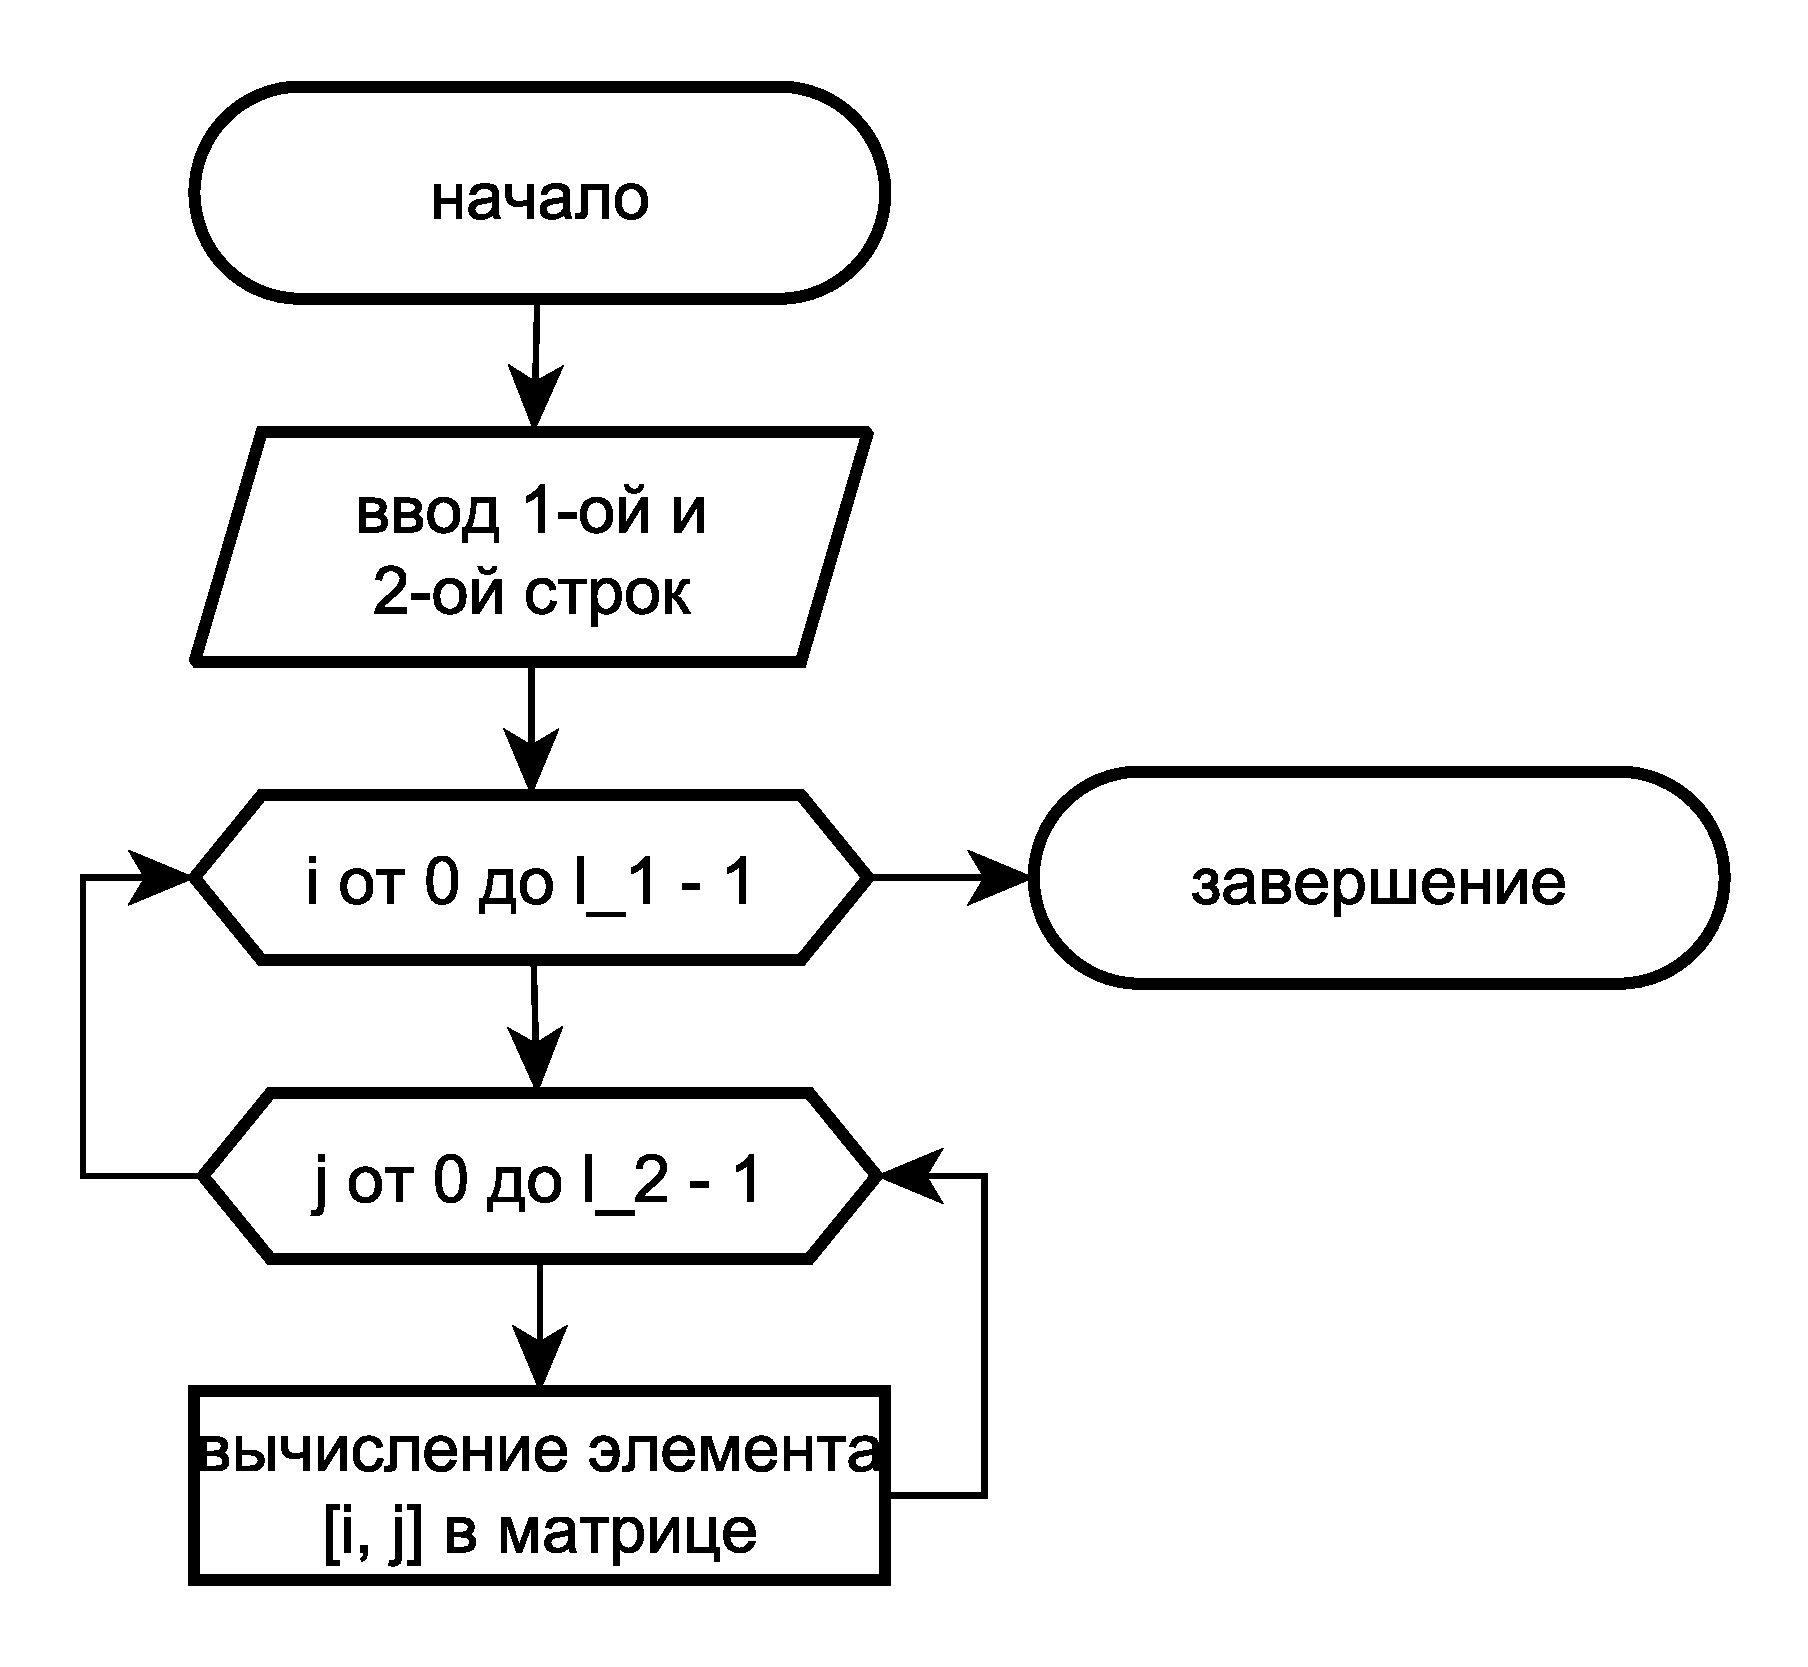
\includegraphics[width = 0.85\textwidth]{flowchart_1}
\captionof{figure}{Схема алгоритма функции поиска расстояния Левенштейна}
\label{fig:label1}


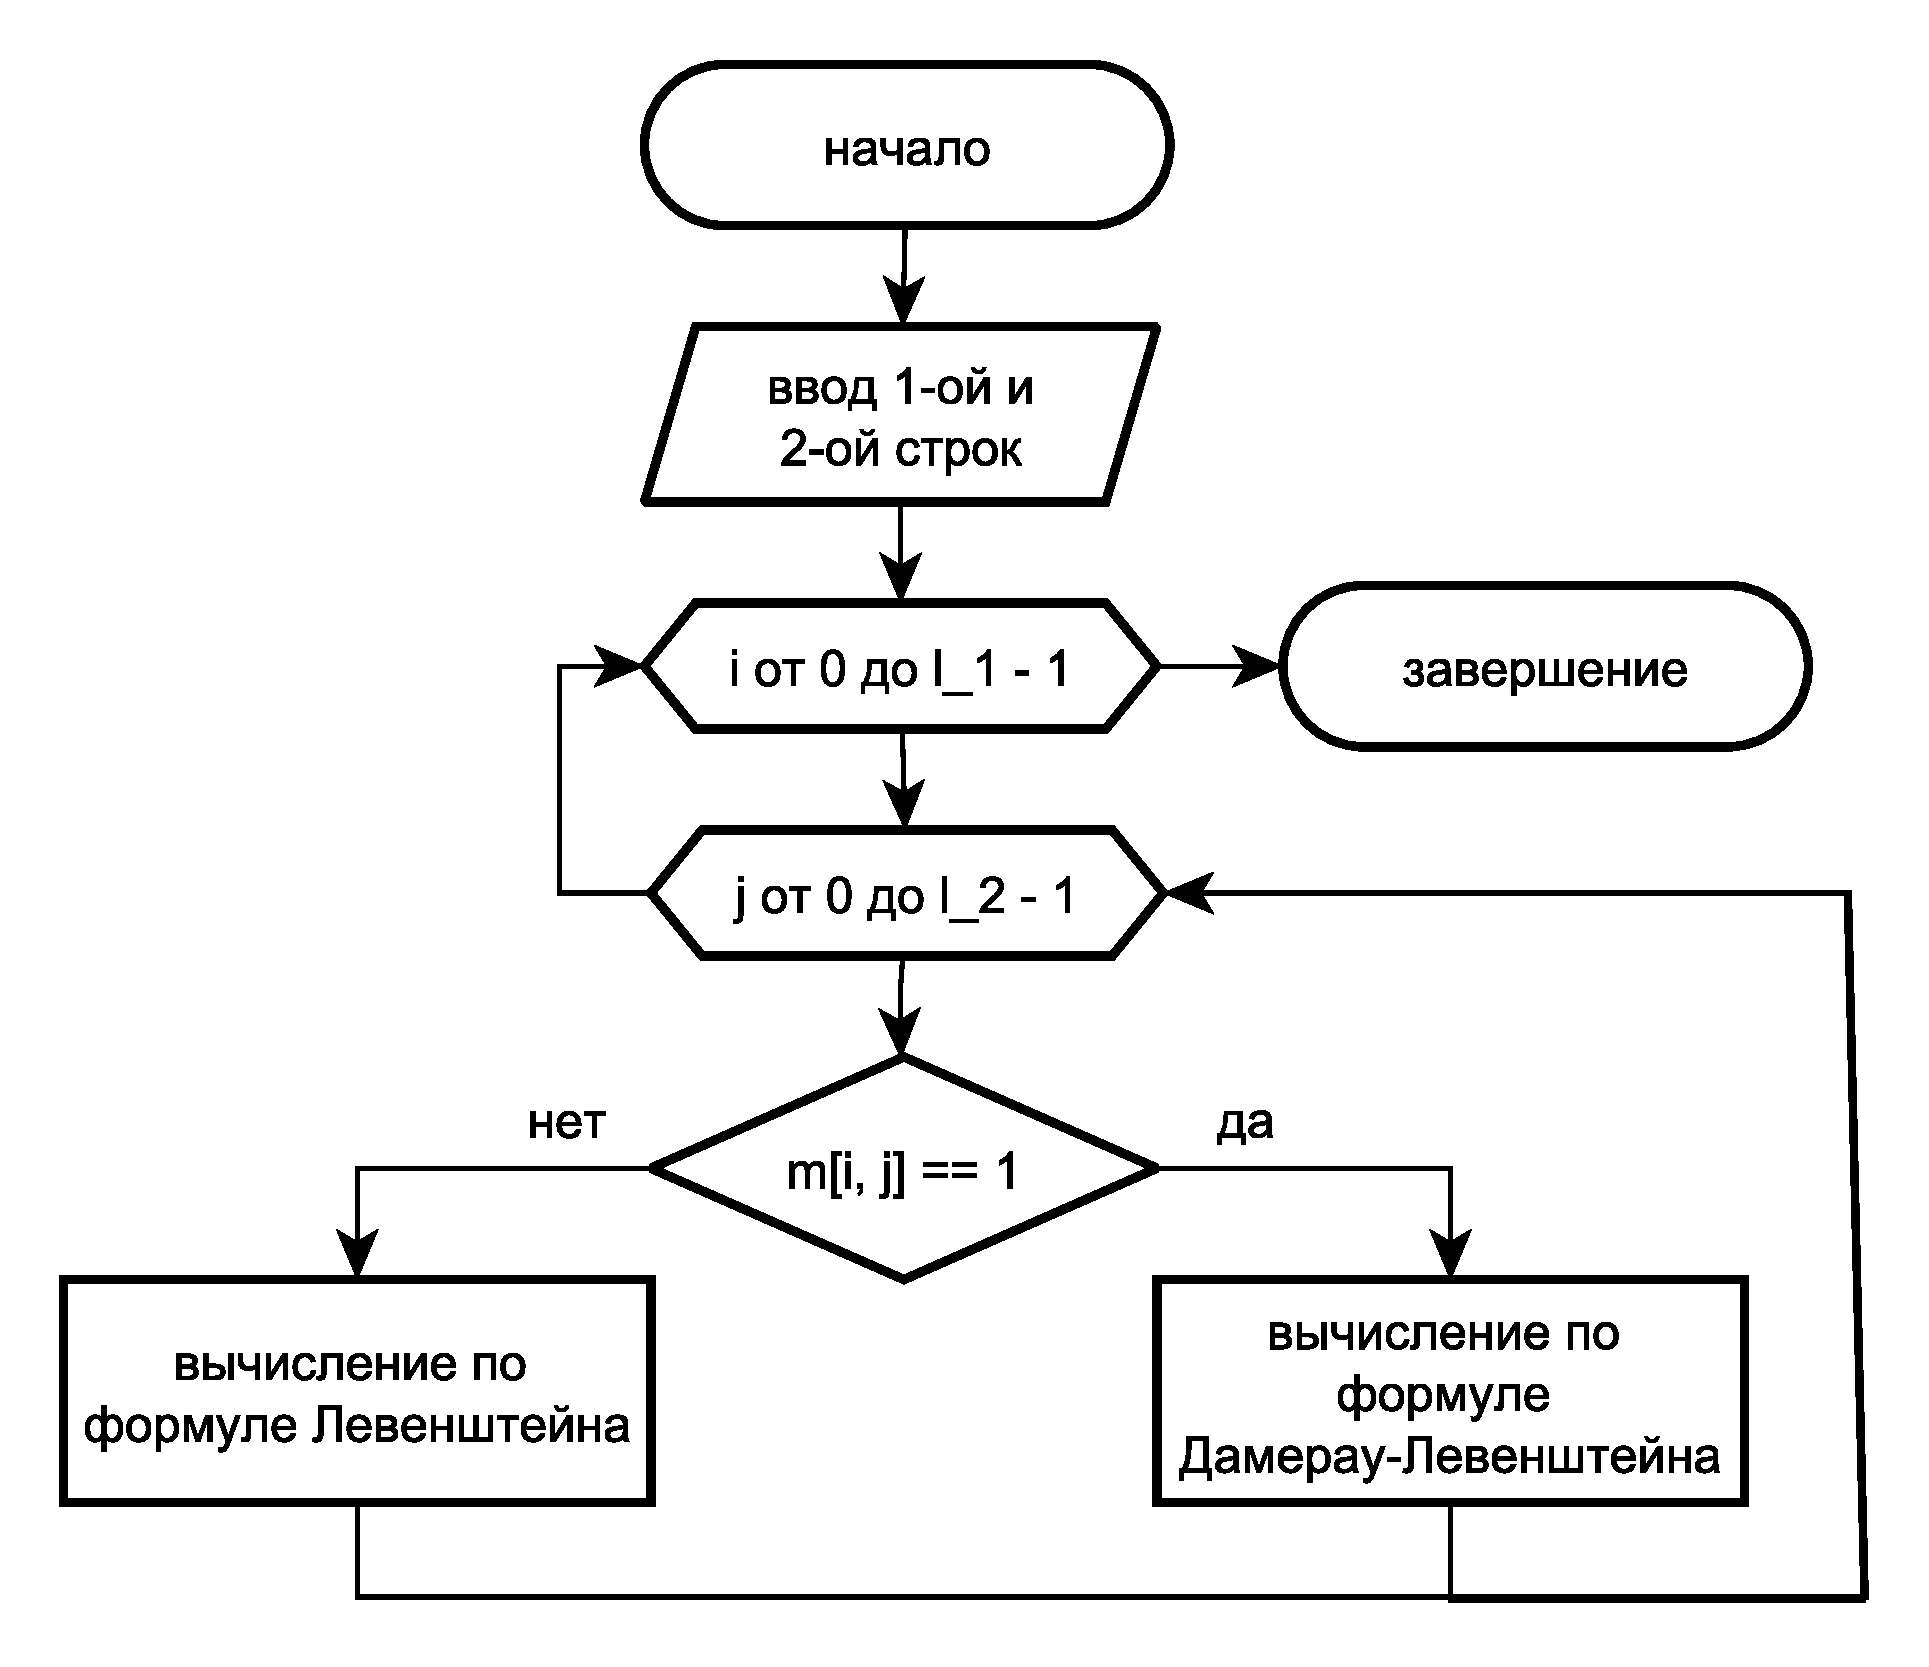
\includegraphics[width = 0.85\textwidth]{flowchart_2}
\captionof{figure}{Схема алгоритма функции поиска расстояния Дамерау--Левенштейна}
\label{fig:label2}

\newpage
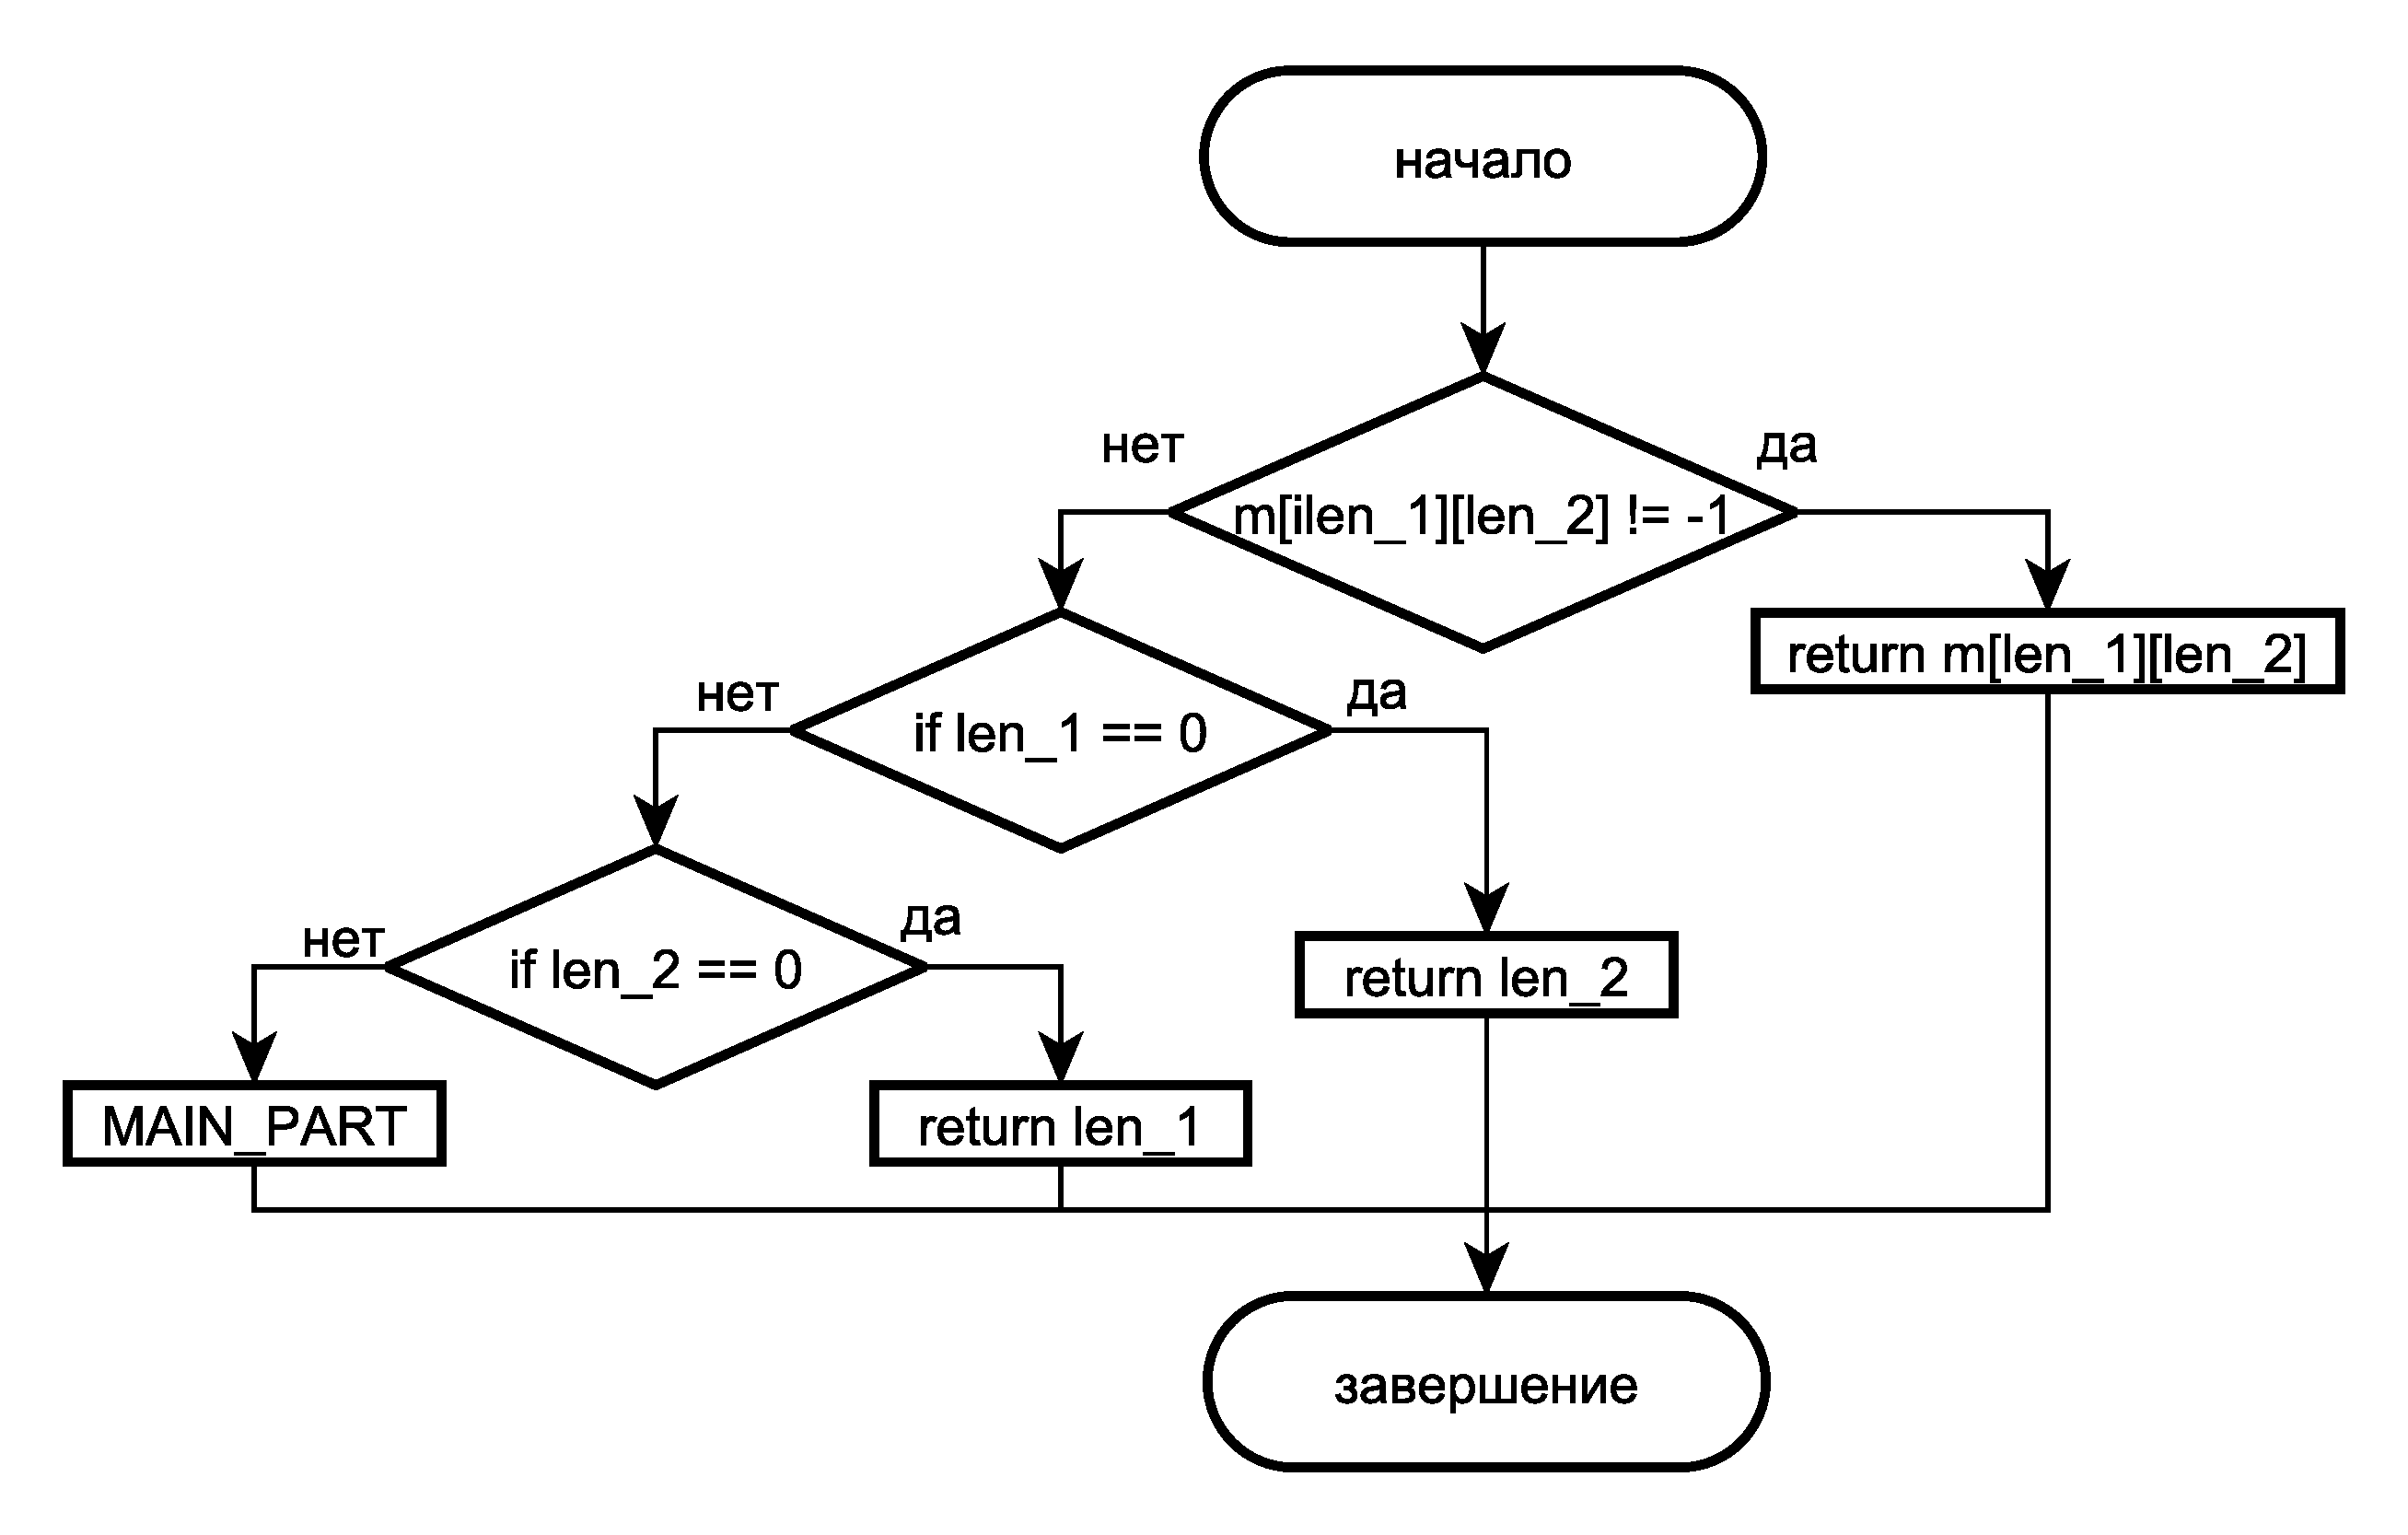
\includegraphics[width = 0.85\textwidth]{flowchart_3}
\captionof{figure}{Схема рекурсивного алгоритма поиска расстояния Левенштейна}
\label{fig:label3}
\end{center}

Подпрограмма MAIN\_PART выполняет следующую работу: return min(alg (str\_1, str\_2, len\_2, len\_1 - 1) + 1, alg(m, len\_2 - 1, len\_1) + 1, alg(m, len\_2 - 1, len\_1 - 1) + n), где alg --- рекусивный алгоритм.

\newpage
Рекурсивный алгоритм с кэшем поиска редакционного расстояния, основанный на формуле нахождения расстояния Левенштейна представлен на схеме алгоритма на рисунок~\ref{fig:label4}.
Рекурсивный алгоритм для расстояния Дамерау-Левенштейна аналогичен и отличен только тем, что при $m_{i,j} == 1$, часть MAIN\_PART примет вид:
return min(alg(str\_1, str\_2, len\_2, len\_1 - 1) + 1, alg(str\_1, sre\_2, len\_2 - 1, len\_1) + 1,
alg(str\_1, str\_2, len\_2 - 1, len\_1 - 1) + n, \\
alg(str\_1, str\_2, len\_2 - 2, len\_1 - 2) + 1);  

\begin{center}
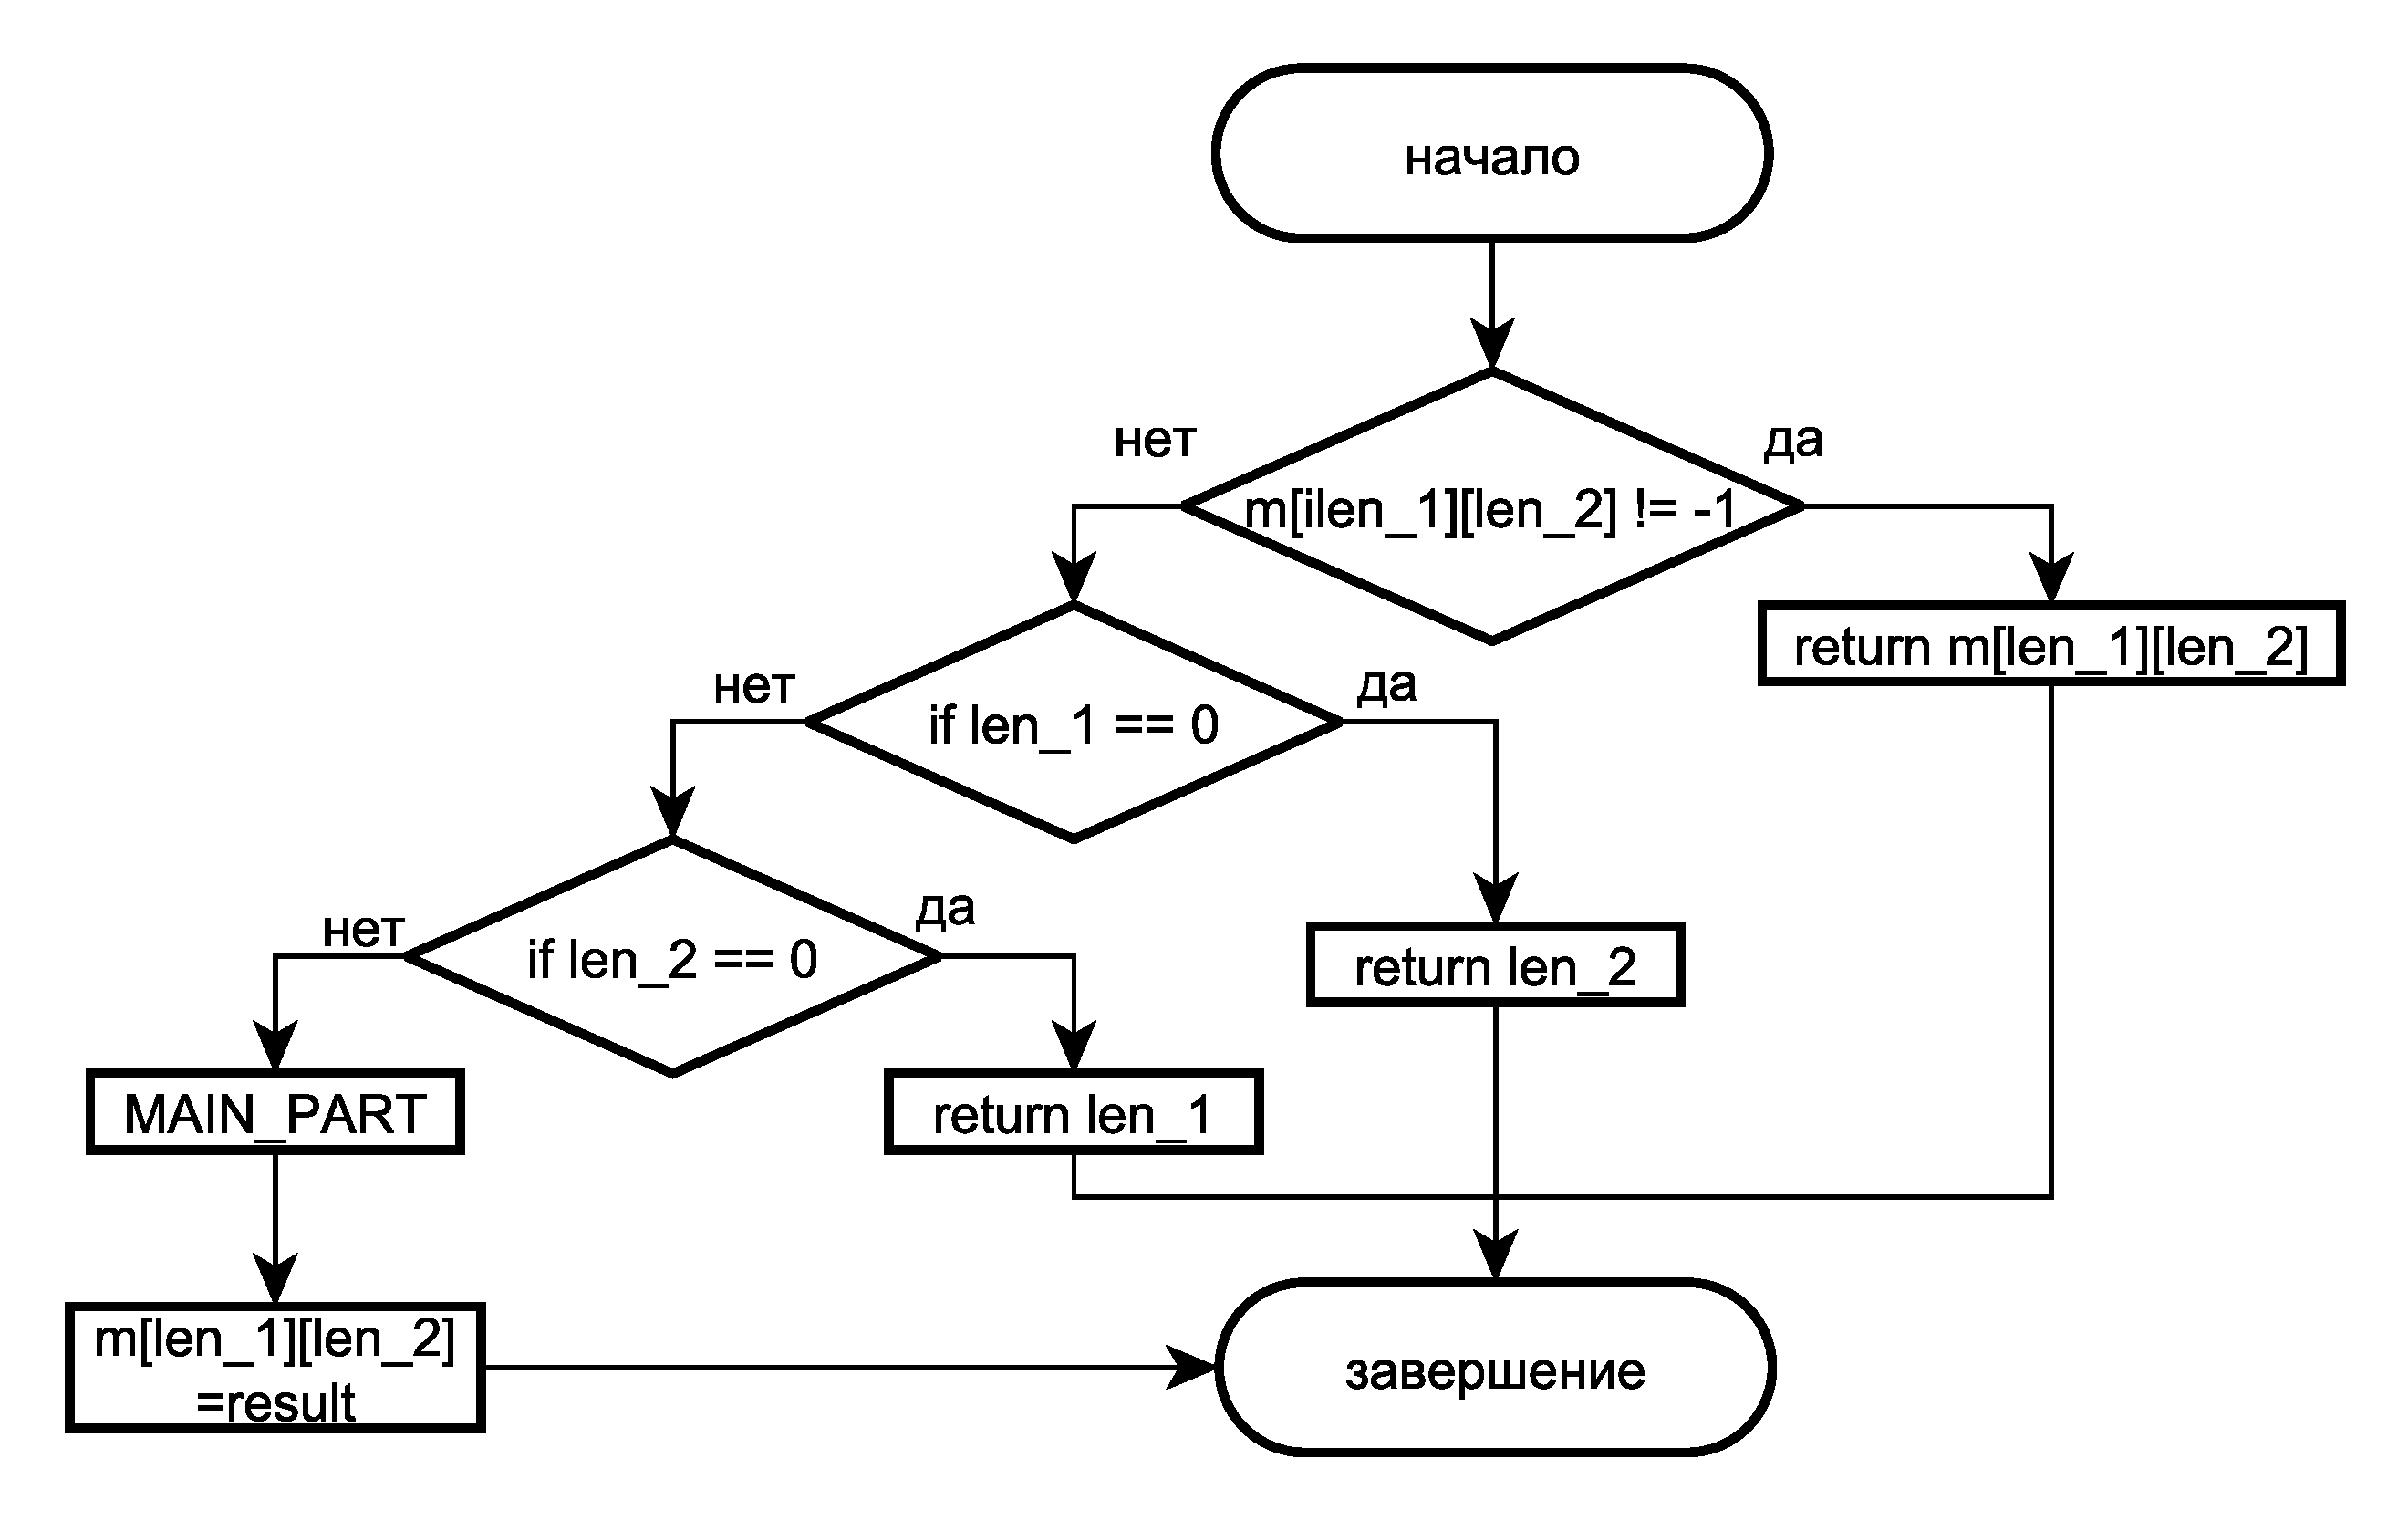
\includegraphics[width = 0.85\textwidth]{flowchart_4}
\captionof{figure}{Схема алгоритма функции рекурсивного алгоритма поиска растояния Левенштейна с кэшем}
\label{fig:label4}
\end{center}

\newpage
\subsection{Анализ сложностей} 
В таблице~\ref{tab:chara} представлены асимптотические сложности разобранных алгоритмов по времени и по памяти. Рекурсивный алгоритм затрачивает на порядок больше времени для вычисления (таблица№1) относительно обычному алгоритму и алгоритму с кэшем. А обычный алгоритм и алгоритм с кэшем затрачивают одинаковое количество ресурсов, что по памяти, что по времени.
\begin{table}[htbp]
	\centering
	\caption{Асимптотические сложности разобранных алгоритмов}
	\begin{tabular}{|c|c|c|}
		\hline
		Алгоритм & Сложность по времени & Сложность по памяти \\
		\hline
		Поиск расстояния& $O(n\cdot m)$ &  $O(n\cdot m)$\\
		Левенштейна&&\\
		\hline
		Поиск расстояния & $O(n\cdot m)$ &  $O(n\cdot m)$\\
		Дамерау--Левенштейна &&\\
		\hline
		Рекурсивный алгоритм& $O(4^{max(n, m)})$ & $O(n\cdot m + 20\cdot(n+m))$\\
		Поиска расстояния &&\\
		Дамерау--Левенштейна&&\\ 
		\hline
		Рекурсивный алгоритм& $O(n\cdot m)$ & $O(n\cdot m)$\\
		c кэшем&&\\
		\hline
	\end{tabular}
	\label{tab:chara}
\end{table}

\newpage

\section{Технологическая часть} 
\subsection{Выбор средств реализации}
Для программной реализации использовалась среда разработки Visual Studio, язык программирования, на котором была выполнена реализации --- C++. 
Исследование проводилось на ноутбуке (64-разрядная операционная система, процессор x64, частота процессора 3.10~Ггц, оперативная память 16~ГБ)\par
Для замера времени использовались функции библиотеки Chrono~[\ref{s:2}].


\subsection{Реализация алгоритмов}
В листинге~\ref{list1} можно увидеть программную реализацию описанных алгоритмов.
\lstset{
    language=C++,
    basicstyle=\ttfamily\fontsize{12}{14}\selectfont,
    breaklines=true,
    keywordstyle=\color{blue},
    commentstyle=\color{gray},
    stringstyle=\color{red},
    postbreak=\mbox{\textcolor{red}{$\hookrightarrow$}\space},
    showstringspaces=false,
    keepspaces=true,
     numbers=left,              
    numberstyle=\tiny,           
    stepnumber=1,                 
    numbersep=5pt,               
    backgroundcolor=\color{white},
    frame=single,  
}


\begin{lstlisting}[label = list1, caption = програмная реализация вспомогательной структуры]
struct matrix {
	public:
	matrix(string str_1, string str_2) {
		this->rows = (str_2.size() + 1);
		this->columns = (str_1.size() + 1);
		this->str_1 = "_" + str_1;
		this->str_2 = "_" + str_2;
		this->c = new int* [rows];
		prepair_matrix();
	}
	
	~matrix() {
		delete[] c;
	}
	
	void print() {
		cout << setiosflags(ios::left);
		
		for (int i = 0; i < rows; i++) {
			cout << setw(2) << "|";
			for (int j = 0; j < columns; j++) {
				cout << setw(3) << c[i][j] << " ";
			}
			cout << "|" << endl;
		}
	}
	
	int* operator[] (int row) {
		return (this->c[row]);
	}
	
	string str(int ind) {
		if (ind == 1) {
			return str_1;
		}
		return str_2;
	}
	
	int ro() {
		return rows;
	}
	
	int co() {
		return columns;
	}
	
	private:
	string str_1;
	string str_2;
	int rows;
	int columns;
	int** c;
	
	void prepair_matrix() {
		for (int i = 0; i < rows; i++) {
			c[i] = new int[columns];
			for (int j = 0; j < (columns); j++) {
				if (i == 0) {
					c[i][j] = j;
				}
				else if (j == 0) {
					c[i][j] = i;
				}
				else {
					c[i][j] = -1;
				}
			}
		}
	}
};
\end{lstlisting}

\newpage
\begin{lstlisting}[label = list2, caption = Программная реализация разработанных алгоритмов]
void aloritm_Lev(matrix* m) {
	int n;
	for (int i = 0; i < (*m).ro(); i++) {
		for (int j = 0; j < (*m).co(); j++) {
			//formula for finding the Levenshtein distance
			if (i == 0) {
				(*m)[i][j] = j;
			}
			else if (j == 0) {
				(*m)[i][j] = i;
			}
			else {
				if ((*m).str(2)[i] == (*m).str(1)[j]) n = 0;
				else n = 1;
				(*m)[i][j] = min(min((*m)[i][j - 1] + 1, (*m)[i - 1][j] + 1), ((*m)[i - 1][j - 1] + n));
			}
		}
	}
}

void algoritm_Dam_Lev(matrix* m) {
	int n;
	for (int i = 0; i < (*m).ro(); i++) {
		for (int j = 0; j < (*m).co(); j++) {
			if (i == 0) {
				(*m)[i][j] = j;
			}
			else if (j == 0) {
				(*m)[i][j] = i;
			}
			else {
				if ((*m).str(2)[i] == (*m).str(1)[j]) n = 0;
				else n = 1;
				if ((j > 1) && (i > 1) && ((*m).str(2)[i] == (*m).str(1)[j - 1]) && ((*m).str(2)[i - 1] == (*m).str(1)[j])) {
					(*m)[i][j] = min(min((*m)[i][j - 1] + 1, (*m)[i - 1][j] + 1), min((*m)[i - 1][j - 1] + n, (*m)[i - 2][j - 2] + 1));
				}
				else {
					(*m)[i][j] = min(min((*m)[i][j - 1] + 1, (*m)[i - 1][j] + 1), (*m)[i - 1][j - 1] + n);
				}
			}
		}
	}
}

int alg_Lev_rec(matrix* m, int len_2, int len_1) {
	int n;
	
	//formula for finding the Levenshtein distance by recirsion
	if (len_1 == 0) {
		return len_2;
	}
	else if (len_2 == 0) {
		return len_1;
	}
	else {
		if ((*m).str(2)[len_2] == (*m).str(1)[len_1]) n = 0;
		else n = 1;
		return min(min(alg_Lev_rec(m, len_2, len_1 - 1) + 1, alg_Lev_rec(m, len_2 - 1, len_1) + 1), alg_Lev_rec(m, len_2 - 1, len_1 - 1) + n);
	}
}

int alg_Dam_Lev_rec(matrix* m, int len_2, int len_1) {
	int n;
	
	//formula for finding the Levenshtein distance by recirsion
	if (len_1 == 0) {
		return len_2;
	}
	else if (len_2 == 0) {
		return len_1;
	}
	else {
		if ((*m).str(2)[len_2] == (*m).str(1)[len_1]) n = 0;
		else n = 1;
		if ((len_1 > 1) && (len_2 > 1) && ((*m).str(2)[len_2] == (*m).str(1)[len_1 - 1]) && ((*m).str(2)[len_2 - 1] == (*m).str(1)[len_1])) {
			return min(min(alg_Dam_Lev_rec(m, len_2, len_1 - 1) + 1, alg_Dam_Lev_rec(m, len_2 - 1, len_1) + 1), min(alg_Dam_Lev_rec(m, len_2 - 1, len_1 - 1) + n, alg_Dam_Lev_rec(m, len_2 - 2, len_1 - 2) + 1));
		}
		return min(min(alg_Dam_Lev_rec(m, len_2, len_1 - 1) + 1, alg_Dam_Lev_rec(m, len_2 - 1, len_1) + 1), alg_Dam_Lev_rec(m, len_2 - 1, len_1 - 1) + n);
	}
}

int alg_Lev_rec_cash(matrix* m, int len_2, int len_1) {
	if ((*m)[len_2][len_1] != -1) {
		return (*m)[len_2][len_1];
	}
	
	int n;
	if (len_1 == 0) {
		return len_2;
	}
	else if (len_2 == 0) {
		return len_1;
	}
	else {
		if ((*m).str(2)[len_2] == (*m).str(1)[len_1]) {
			n = 0;
		}
		else {
			n = 1;
		}
		
		(*m)[len_2][len_1] = min(min(alg_Lev_rec_cash(m, len_2, len_1 - 1) + 1, alg_Lev_rec_cash(m, len_2 - 1, len_1) + 1), alg_Lev_rec_cash(m, len_2 - 1, len_1 - 1) + n);
		return (*m)[len_2][len_1];
	}
}
\end{lstlisting}

\newpage
\subsection{Тестирование программы}

В таблице~\ref{tab:tests} представлены описания тестов по методологии чёрного ящика, все тесты пройдены успешно.

\begin{table}[htbp]
	\centering
	
	\caption{Описание тестов по методологии чёрного ящика}
	\begin{tabular}{|p{0.05\linewidth}|p{0.2\linewidth}|p{0.12\linewidth}|p{0.25\linewidth}|p{0.25\linewidth}|}
		\hline
		& \textbf{Описание теста} & \textbf{Входные данные} & \textbf{Ожидаемый результат} & \textbf{Полученный результат} \\
		\hline
		
		\textbf{1} & проверка на обработку не валидных данных & 3 & оповещение о некорректности данных и запрос новых & оповещение о некорректности данных и запрос новых \\
		\hline
		
		\textbf{2} & проверка на коректность работы алгоритмов & 1\newline 123456 \newline 132546 &Левенштейн: 3 \newline Дамерау-Левенштейн: 2 \newline
		&Левенштейн: 3 \newline Дамерау-Левенштейн: 2\\
		\hline
		
		\textbf{3} & проверка на единичные строки & 1\newline 
		2\newline 2&Левенштейн: 0 \newline Дамерау-Левенштейн: 0 \newline
		& Левенштейн: 0 \newline Дамерау-Левенштейн: 0 \\
		\hline
		
		\textbf{4} & проверка на коректность работы с матрицей 1 на n & 1\newline 1 \newline 123456 &Левенштейн: 5 \newline Дамерау-Левенштейн: 5 \newline
		&Левенштейн: 5 \newline Дамерау-Левенштейн: 5 \\
		\hline
		
	\end{tabular}
	\label{tab:tests}
\end{table}

\newpage
\section{Исследовательская часть}
\subsection{Замеры процессорного времени выполнения реализации алгоритмов}
На рисунке~\ref{grh:1} можно увидеть графики, иллюстрирующие зависимость процессорного времени выполнения реализации алгоритма расчета редакционного расстояния от длины строки для рекурсивного алгоритма и для обычного с кэшем. Пусть длины строк совпадают.

\begin{center}
\includegraphics[width = 0.9\textwidth]{chart_1}
\captionof{figure}{Визуализация зависимости процессорного времени при выполнении реализации рекурсивного и обычного алгоритма поиска расстояния Левенштейна от длины строк.}
\label{grh:1}
\end{center}

Из этого можно сделать вывод, что рекурсивный алгоритм намного более затратный с точки зрения числа выполненных операций (затраченного на расчёт времени). Так, для строк длиной 7 затрачено в 140 раз больше времени. \par % тут пример для конкретной пары точек с графика
\newpage

Визуализацию проведенного замеров затрачиваемого процессорного времени обычным алгоритмом с кэшем и рекурсивным с кэшем, можно увидеть на рисунке~\ref{grh:2}.\par

\begin{center}
\includegraphics[width=0.9\textwidth]{chart_2}
\captionof{figure}{Визуализация зависимости процессорного времени выполнения реализации рекурсивного с кэшем и обычного алгоритмов поиска расстояния Левенштейна от длины строк.}
\label{grh:2}
\end{center}

Проанализировав графики, можно отметить, что процессорное время, затрачиваемое на выполнение реализации алгоритмов поиска расстояния Дамерау -- Левенштейна, как рекурсивного с кэшем, так и нерекурсивного, намного меньше, чем то время, которое затрачивается на выполнение реализации рекурсивного алгоритма поиска расстояния Левенштейна даже на строках маленькой длины.

Рекурсивный алгоритм с кэшем и обычный алгоритм с кэшем показывают примерно равные результаты.

\newpage
\section*{ЗАКЛЮЧЕНИЕ}
\addcontentsline{toc}{section}{ЗАКЛЮЧЕНИЕ}
%\subsection*{Вывод}
В результате лабораторной работы были выполнены все поставленные задачи.
\begin{enumerate}
    \item Описана математическая основа расстояния Левенштейна и Дамерау---Левен\-штейна,
    \item Описана модель вычисления,
    \item Реализована программу для расчёта расстояний Дамерау-Левенштейна и Левенштейна,
    \item Выполнена оценка трудоёмкости реализации алгоритмов,
    \item Реализованы разработанные алгоритмы в программном обеспечении с двумя режимами работы -- одиночного расчёта и массированного замера процессорного времени,
    \item Выполнены замеры процессорного времени выполнения реализации каждого алгоритма в зависимости от длины строк,
    \item Выполнен сравнительный анализ рассчитанных трудоёмкостей и результатов замера процессорного времени,
\end{enumerate}

Цель работы достигнута: выполнена оценка ресурсной эффективности алгоритмов нахождения расстояния Левенштейна и Дамерау---Левенштейна.



\newpage
\section*{СПИСОК ИСПОЛЬЗОВАННЫХ ИСТОЧНИКОВ}

\addcontentsline{toc}{section}{СПИСОК ИСПОЛЬЗОВАННЫХ ИСТОЧНИКОВ}
\begin{list}{\arabic{enumi}.}{\usecounter{enumi} \leftmargin=0pt \rightmargin=0pt}
	\item \justifying Ульянов М. В. Ресурсно эффективные компьютерные алгоритмы / Учебное пособие 2007.\label{s:1}
	
	\item \justifying Microsoft. GetProcessTimes function. [Электронный ресурс] - URL:https://learn.microsoft.com/ru-ru/cpp/standard-library/processthreadsapi/chrono \par
	(дата обращения: 20.09.2024).\label{s:2}
	
	\item \justifying AlgoLib. [Электронный ресурс] - URL: https://www.algolib.narod/Math/Matrix \par
	(дата обращения: 20.09.2024).\label{s:3}
\end{list}

\end{document}
